\pdfoutput=1
\documentclass[11pt]{amsart}
\usepackage{amsmath,amssymb,amsthm,mathtools}
\usepackage[margin=1.2in]{geometry}
\usepackage{graphicx,booktabs,adjustbox,tikz}
\usetikzlibrary{arrows.meta,positioning}
\usepackage{xcolor}
\usepackage[colorlinks=true,linkcolor=blue,citecolor=blue,urlcolor=blue]{hyperref}
\hypersetup{pdfauthor={Bernd Johannes Wuebben},
  pdftitle={Uniform Hermitian--Einstein spectra for bipartite two-step extensions}}
\newtheorem{theorem}{Theorem}[section]
\newtheorem{proposition}[theorem]{Proposition}
\newtheorem{lemma}[theorem]{Lemma}
\newtheorem{corollary}[theorem]{Corollary}
\theoremstyle{definition}
\newtheorem{definition}[theorem]{Definition}
\newtheorem{example}[theorem]{Example}
\newtheorem{question}[theorem]{Question}
\theoremstyle{remark}
\newtheorem{remark}[theorem]{Remark}
\setlength{\emergencystretch}{2em}
\newcommand{\db}{\bar\partial}
\newcommand{\End}{\operatorname{End}}
\newcommand{\Hom}{\operatorname{Hom}}
\newcommand{\Ext}{\operatorname{Ext}}
\newcommand{\tr}{\operatorname{tr}}
\newcommand{\rk}{\operatorname{rk}}
\newcommand{\diag}{\operatorname{diag}}
\newcommand{\id}{\operatorname{id}}
\newcommand{\osc}{\operatorname{osc}}
\newcommand{\capk}{\operatorname{cap}}
\newcommand{\RR}{\mathbb R}
\newcommand{\CC}{\mathbb C}
\newcommand{\PP}{\mathbb P}
\newcommand{\HH}{\mathcal H}
\newcommand{\cC}{\mathcal C}
\newcommand{\cR}{\mathcal R}
\newcommand{\one}{\mathbf 1}
\title[Uniform spectra near stability walls]{Uniform Hermitian--Einstein spectra\\for bipartite two-step extensions}
\author{Bernd Johannes Wuebben}
\subjclass[2020]{53C07 (primary); 53C55, 58J50, 05C50 (secondary)}
\keywords{Hermitian--Einstein metric, slope stability, Dolbeault Laplacian,
  vector bundle extension, weighted graph Laplacian, stability wall}
\date{October 27, 2026}
\begin{document}
\begin{abstract}
We determine the complete small spectrum of Hermitian--Einstein bundles
near intersections of slope-stability walls. Consider a fixed extension of
one direct sum of stable bundles by another, with pairwise nonisomorphic
factors of equal slope at the reference Kähler form. Assume that its
nonzero extension components have connected support. In the local stable
chamber, the small eigenvalues of the Dolbeault Laplacian on trace-free
endomorphisms agree with those of a balanced, rank-weighted graph
Laplacian to relative error \(O(\sigma)\), where \(\sigma\) is the total
balanced conductance. The estimate holds for every small eigenvalue,
uniformly through arbitrary positive ratios of the stability margins,
and the remaining spectrum has a uniform gap.

The construction uses exact curvature identities on graph cuts. These
control the nonlinear error relative to each cut capacity and give an
actual Hermitian--Einstein metric even when the ordinary inverse of the
finite Laplacian is unbounded. We also obtain a relative metric
approximation, coefficient-stability estimates, and a spanning-tree
formula for the product of the small eigenvalues. Trees have
slope-determined leading weights, whereas cyclic supports retain
harmonic extension data.
\end{abstract}
\maketitle
\enlargethispage{5pt}


% ============================================================
% section_01_introduction.tex
% ============================================================
\section{Introduction}\label{sec01:introduction}

A strictly semistable bundle may have a graded object with more
endomorphisms than the original bundle. As a stable polarization
approaches the corresponding wall, these additional endomorphisms
appear analytically as almost-holomorphic endomorphisms with small
Dolbeault energy. The question is then quantitative: how many small
eigenvalues occur, and how fast does each one vanish?

At an intersection of walls, there need not be one degeneration scale.
One stability margin may be much smaller than all the others. An
absolute spectral error, even one of higher order in the total
distance to the wall, may then be larger than the smallest eigenvalue.
We seek relative estimates for every small eigenvalue, with no lower
bound on the ratios between the positive margins.

The bundles considered here are two-step extensions. Their stable
factors form the vertices of a bipartite graph, and a nonzero extension
component gives an arrow from a quotient factor to a subbundle factor.
The effective operator is a weighted graph Laplacian. Its vertex
masses are the factor ranks; its edge conductances are obtained by
balancing the harmonic norms of the extension components against the
slope defects. The main point is to justify this operator uniformly
for actual Hermitian--Einstein metrics as any collection of positive
cut margins becomes small relative to the others.

\subsection{The setting and the effective operator}

Let \(X\) be a compact connected Kähler manifold of complex dimension
\(n\geq1\), and let \(\omega_s\), \(s\in U\subset\RR^a\), be a smooth
family of Kähler forms with reference parameter \(s=0\).
Fix holomorphic vector bundles \(F_1,\ldots,F_m\), \(m\geq2\), which
are pairwise nonisomorphic, stable, and of equal slope at \(\omega_0\).
Choose a partition \(I\sqcup J=\{1,\ldots,m\}\) and a fixed extension
\begin{equation}\label{eq01:extension}
 0\longrightarrow S=\bigoplus_{i\in I}F_i
 \longrightarrow E
 \longrightarrow U_0=\bigoplus_{j\in J}F_j
 \longrightarrow0.
\end{equation}
We use \emph{two-step} to refer to this extension of a direct sum by a
direct sum. In particular, arrows are not composable.

The support graph \(\Gamma\) has vertex set \(\{1,\ldots,m\}\) and an
edge \(e:j\to i\) exactly when the corresponding class in
\(\Ext^1(F_j,F_i)\) is nonzero. There is one edge for each nonzero
matrix block, not for each basis vector of that Ext group.
Write \(\Gamma(0)\) and \(\Gamma(1)\) for its vertex and edge sets,
and \(s(e)\), \(t(e)\) for the source and target of an edge.
We assume that the underlying undirected graph is connected.
A cycle will always mean an undirected cycle in this bipartite graph.

Write \(r_v=\rk F_v\), \(R=\sum_vr_v\), and
\begin{equation}\label{eq01:normalization}
\begin{aligned}
 V_s&=\int_X\frac{\omega_s^n}{n!},&
 \deg_s F&=\int_Xc_1(F)\frac{\omega_s^{n-1}}{(n-1)!},\\
 \kappa_v(s)&=\frac{2\pi\deg_s F_v}{V_sr_v},&
 \kappa_E(s)&=\frac1R\sum_vr_v\kappa_v(s).
\end{aligned}
\end{equation}
All stability notions are slope stability:
\(\mu_s(F)=\deg_s(F)/\rk F\), and stability requires a strict
slope inequality for every coherent subsheaf of positive rank
smaller than the bundle rank.
The centered slope demands are
\begin{equation}\label{eq01:demands}
 b_v(s)=-r_v\bigl(\kappa_v(s)-\kappa_E(s)\bigr),
 \qquad \sum_v b_v(s)=0.
\end{equation}
If \(D\) is the incidence matrix with column \(D_e=e_i-e_j\)
for \(e:j\to i\), define
\[
 \cC=D\RR_{\geq0}^{\Gamma(1)},\qquad
 \cC^\circ=D\RR_{>0}^{\Gamma(1)}.
\]
Connectedness makes \(\cC^\circ\) the interior of \(\cC\) in the
zero-sum vertex hyperplane. We prove the relevant cone
characterization below.
A vertex subset \(C\) is an ideal if no arrow leaves it; its
stability margin is \(b_C=\sum_{v\in C}b_v\).
The proper nonempty ideal margins are precisely the inequalities
which will characterize this cone.

Continue normalized factor Hermitian--Einstein metrics \(h_{v,s}\)
smoothly from the reference parameter, and let \(\beta_{e,s}\) be
the representative of the fixed nonzero extension component which is
harmonic for \(\omega_s\) and the metrics
\(h_{t(e),s},h_{s(e),s}\). Set
\begin{equation}\label{eq01:coefficients}
 c_e(s)=\frac{\|\beta_{e,s}\|_{L^2_s}^2}{V_s}>0.
\end{equation}
The continuation and the fixed-bundle harmonic identifications are
included in the construction below. After shrinking \(U\), all
coefficients have a common positive lower bound.

For \(b\in\cC^\circ\), there is a unique positive edge vector
\begin{equation}\label{eq01:balance}
 k_e(s,b)=c_e(s)\exp\bigl((D^Tx_0)_e\bigr),\qquad
 Dk=b,\qquad \sum_vr_v(x_0)_v=0.
\end{equation}
The potential \(x_0\) is normalized here by rank-weighted mean zero;
the edge vector does not depend on that normalization.
The effective operator is
\begin{equation}\label{eq01:graphoperator}
 A(k)=M^{-1/2}D\diag(k)D^TM^{-1/2},
 \qquad M=\diag(r_1,\ldots,r_m).
\end{equation}
It has one zero eigenvalue. Denote its positive eigenvalues by
\(\nu_1(k)\leq\cdots\leq\nu_{m-1}(k)\), with multiplicity.
Equivalently, these are the eigenvalues for the energy and mass
\begin{equation}\label{eq01:energy}
 q_k(x)=\sum_e k_e|x_{t(e)}-x_{s(e)}|^2,\qquad
 \|x\|_M^2=\sum_vr_v|x_v|^2,\qquad
 \sum_vr_vx_v=0.
\end{equation}

\subsection{Uniform relative asymptotics}

For a Hermitian metric \(h\) on \(E\), our elliptic operator is
\[
 \Delta_{h,s}=\db_{\End E}^{*_{h,\omega_s}}\db_{\End E}
 \quad\hbox{on }\End_0E.
\]
Here \(\End_0E\) denotes pointwise trace-free complex endomorphisms,
and spectral multiplicities are complex. This operator is not the
full Yang--Mills Hessian.

\begin{theorem}\label{thm01:main}
There are a neighborhood of \(0\) and constants \(C,\gamma>0\),
depending on the fixed data above, with the following properties.
The fixed bundle \(E\) is stable at \(s\) if and only if
\(b(s)\in\cC^\circ\).
In that chamber let \(h_{\mathrm{HE},s}\) be its
Hermitian--Einstein metric and put
\begin{equation}\label{eq01:sigma}
 \sigma(s)=\sum_e k_e(s,b(s))
          =\sum_{i\in I}b_i(s)>0.
\end{equation}
Its endomorphism Dolbeault spectrum satisfies
\begin{equation}\label{eq01:mainestimate}
 \left|\frac{\lambda_j(h_{\mathrm{HE},s})}
                 {\nu_j(k(s,b(s)))}-1\right|
 \leq C\sigma(s)\quad(1\leq j<m),\qquad
 \lambda_m(h_{\mathrm{HE},s})\geq\gamma.
\end{equation}
Thus there are exactly \(m-1\) eigenvalues tending to zero.
The constants are independent of all ratios between positive
conductances, positive ideal margins, or small eigenvalues.
In particular, the demand
direction may approach any face or intersection of faces of
\(\cC\) at arbitrary relative rates.
\end{theorem}

The theorem concerns one fixed extension. It does not give constants
uniform in extension classes tending to zero, changing support
graphs, or increasing numbers of vertices. It allows a
finite-dimensional family of forms, including tangential parameter
directions; it does not assume \(|s|=O(\sigma(s))\).
If the chosen parameter family has no stable points, the chamber
assertions are empty.

The construction also gives a metric approximation. Let \(\Phi_s\)
identify the fixed extension with its amplitude-one harmonic
presentation, let \(h_{0,s}=\bigoplus_vh_{v,s}\), and set
\[
 g_0=\diag\bigl(e^{(x_0)_v/2}\id_{F_v}\bigr),\qquad
 h_{\mathrm{mod},s}=\Phi_s^*g_0^*h_{0,s}.
\]
With the common determinant normalization, we obtain
\begin{equation}\label{eq01:metric}
 e^{-C\sigma}h_{\mathrm{mod},s}
 \leq h_{\mathrm{HE},s}
 \leq e^{C\sigma}h_{\mathrm{mod},s}.
\end{equation}
The same \(\Phi_s\) occurs in both metrics. The estimate remains
valid when the diagonal weights diverge; it does not freeze the
harmonic splitting while those weights become singular.

\subsection{Why cuts enter the proof}

The complement of the parallel block scalars has a uniform
elliptic gap. Solving the curvature equation there leaves a
finite equation
\begin{equation}\label{eq01:reducedpreview}
 -b+D(c_et_e^2)_e+\cR(s,t)=0.
\end{equation}
The usual expansion gives \(\cR=O(|t|^4)\). That bound alone is
insufficient. For example, on a three-vertex path with conductances
\(q,q^3\), the zero-sum forcing \((0,-q^2,q^2)\) has size
\(O(q^2)\), but its inverse potential has oscillation \(q^{-1}\).
The weakest cut sees an error larger than its conductance.

The geometric equation has more structure. If all amplitudes crossing
a vertex subset \(C\) vanish, the holomorphic bundle and its uniquely
normalized complementary metric split across that cut. Integrated
curvature trace then gives an exact degree identity. A sign symmetry
removes the first crossing derivative. Together these imply
\begin{equation}\label{eq01:cutpreview}
 \left|\sum_{v\in C}\cR_v(s,t)\right|
 \leq C|t|^2\sum_{e\in\partial C}t_e^2
 \quad\hbox{for every cut }C.
\end{equation}
This is a relative estimate at every cut, rather than only at the
scale of the total error. An elementary oscillation estimate for a
graph Laplacian converts it into a uniformly small vertex
correction. A finite-dimensional fixed-point argument then solves
the full Hermitian--Einstein equation. Harmonic cancellation and
min--max give the individual relative spectral estimates.

\subsection{Trees, cycles, and the wider programme}

On a tree, deleting an edge gives a cut which determines that edge's
conductance from \(b\). Thus ranks and slope demands determine the
entire leading spectrum. On a cyclic graph, the equations \(Dk=b\)
leave additional information: the products of harmonic coefficients
around cycles. This information can affect the leading spectrum
even when ranks, slopes, and the chamber agree.

For example, consider a four-cycle with unit vertex masses and
demand \(b=\rho(1,1,-1,-1)\), \(\rho>0\). If
\(\theta=c_{11}c_{22}/(c_{12}c_{21})\), its balanced conductance
matrix is
\[
 (k_{ij})=\rho
 \begin{pmatrix}a&1-a\\1-a&a\end{pmatrix},
 \qquad a=\frac{\sqrt\theta}{1+\sqrt\theta}.
\]
The three positive graph eigenvalues, before ordering, are
\(2\rho a,\,2\rho(1-a),\,2\rho\).
The cycle ratio therefore changes the leading spectral coefficients.
We give the geometric examples and the general cycle identities
after the proof.

The local wall-crossing and convergence theory of
Clarke--Tipler~\cite{clarketipler2024}, the quantitative continuity
theorem of Delloque~\cite{delloque2025}, and the rescaling methods in
Sektnan--Tipler~\cite{sektnantipler2024} provide important analytic
precedents. The last work concerns an adiabatic pullback problem with
its own hypotheses; we do not import that theorem for arbitrary
two-step supports. The star case of the present spectral question
was treated in~\cite{wuebben2026walls}. The contribution here is the
extension to connected non-star bipartite supports, including cycles,
with an actual metric construction uniform through all positive
chamber ratios.

These results are one part of a programme relating stability chambers
to quantitative analytic degeneration. The companion geometric
construction supplies genuine toric tangent bundles with
nonsimplicial chambers. We explain their stationary application
below, with the actual factors, slope coordinates, and harmonic
data specified. Metric-response and flow conclusions require their
own arguments and play no role in the proof of the present theorem.

% ============================================================
% section_02_balancing.tex
% ============================================================
\section{The finite balancing problem}\label{sec02:balancing}

We first isolate the finite problem. This identifies the chamber,
the data retained by cycles, and the estimate needed when the graph
gap becomes small. The arguments apply to any fixed positive
conductances; their constants do not depend on conductance ratios.

\subsection{The positive incidence cone}

A vertex subset \(C\) is an \emph{ideal} for the extension orientation
if an arrow whose source belongs to \(C\) also has its target in
\(C\). Thus no arrow leaves an ideal. Put
\[
 W=\{b\in\RR^m:\one^Tb=0\},\qquad
 b_C=\sum_{v\in C}b_v.
\]

\begin{lemma}\label{lem02:cone}
For a connected bipartite extension graph,
\[
 D\RR_{\geq0}^{\Gamma(1)}
 =\{b\in W:b_C\geq0\text{ for every nonempty proper ideal }C\},
\]
and its interior in \(W\) is
\[
 D\RR_{>0}^{\Gamma(1)}
 =\{b\in W:b_C>0\text{ for every nonempty proper ideal }C\}.
\]
\end{lemma}

\begin{proof}
If \(b=Da\) with \(a\geq0\), summing over an ideal cancels internal
edges and leaves the incoming weights. This proves necessity.
For the converse, the dual cone consists of vertex potentials \(h\)
such that \(D^Th\geq0\). Every upper level set of such an \(h\)
is an ideal. Order its distinct values and express \(h\) as a
constant plus nonnegative multiples of the indicators of its
proper upper level sets. Since \(b\in W\), the constant contributes
zero, and the ideal inequalities imply \(h\cdot b\geq0\).
Separation from the closed finitely generated cone
\(D\RR_{\geq0}^{\Gamma(1)}\) proves the closed-cone assertion.

Connectedness makes every proper cut nonempty. Hence
\(b^0=D\one\) has \(b^0_C>0\) for every proper ideal. If all ideal
sums of \(b\) are positive, choose \(\varepsilon>0\) small enough
that \(b-\varepsilon b^0\) still has nonnegative ideal sums.
Write it as \(Da'\), \(a'\geq0\), and obtain
\(b=D(a'+\varepsilon\one)\) with a strictly positive edge lift.
Conversely every strictly positive lift gives strict ideal sums.
The incidence matrix of a connected graph has rank \(m-1\), so the
positive image is open in \(W\). Conversely, if \(b_C=0\) for
some nonempty proper ideal, then \(b-\varepsilon b^0\) leaves the
closed cone for every \(\varepsilon>0\), so \(b\) is not interior.
This proves the interior statement.
\end{proof}

\subsection{Existence of the balanced weights}

Let \(c_e>0\), \(b\in\cC^\circ\), and choose \(a^0>0\) with
\(Da^0=b\). On the rank-centered hyperplane
\[
 H_M=\{x\in\RR^m:\sum_vr_vx_v=0\}
\]
consider
\begin{equation}\label{eq02:potential}
 \phi_{c,b}(x)=\sum_ec_e e^{(D^Tx)_e}-b\cdot x
 =\sum_e\bigl(c_e e^{(D^Tx)_e}-a_e^0(D^Tx)_e\bigr).
\end{equation}
Each scalar summand is bounded below and tends to infinity as its
argument tends to either end of the real line. Since \(D^T\) is
injective on \(H_M\), the function is coercive there. Its Hessian is
\[
 D\diag\bigl(c_e e^{(D^Tx)_e}\bigr)D^T,
\]
which is positive on every nonconstant direction.
It therefore has a unique minimizer \(x_0\).
Its critical equation is \(Dk=b\): the gradient belongs to \(W\),
while the Euclidean annihilator of \(H_M\) is spanned by
\((r_v)\), whose intersection with \(W\) is zero.
This proves~\eqref{eq01:balance}.

The minimizer need not stay bounded near a chamber face.
Nevertheless, in the bipartite orientation,
\begin{equation}\label{eq02:smallamplitudes}
 \sum_e k_e=\sum_{i\in I}b_i=\sigma,\qquad
 t_e^0=\sqrt{k_e/c_e},\qquad
 \sum_e(t_e^0)^2\leq c_{\min}^{-1}\sigma.
\end{equation}
Thus the harmonic amplitudes, rather than the original vertex
potential, remain uniformly small. This observation allows a
fixed elliptic neighborhood to serve the entire chamber.

\subsection{An inverse estimate measured on cuts}

For any nonempty proper vertex subset \(C\), let
\(\partial C\) consist of all edges with exactly one endpoint in
\(C\). For positive conductances \(k\), define
\[
 \capk_k(C)=\sum_{e\in\partial C}k_e,\qquad
 \|q\|_{\mathrm{cut},k}
 =\max_{\varnothing\ne C\ne\Gamma(0)}
     \frac{|q_C|}{\capk_k(C)}
 \quad(q\in W).
\]
This is a norm on \(W\): the triangle inequality is immediate,
and singleton cuts detect every coordinate. Connectedness
ensures that every denominator is positive.

\begin{lemma}\label{lem02:cutinverse}
Let \(L_k=D\diag(k)D^T\). For any real vertex potential \(y\),
\begin{equation}\label{eq02:cutinverse}
 \|L_ky\|_{\mathrm{cut},k}
 \leq\osc(y)
 \leq(m-1)\|L_ky\|_{\mathrm{cut},k}.
\end{equation}
If \(y\) has zero mean with respect to any positive vertex masses,
then also
\[
 \|y\|_\infty\leq(m-1)\|L_ky\|_{\mathrm{cut},k}.
\]
\end{lemma}

\begin{proof}
For every cut, internal edges cancel and give the
orientation-independent identity
\[
 (L_ky)_C
 =\sum_{\substack{uv\in\partial C\\u\in C,\ v\notin C}}
       k_{uv}(y_u-y_v).
\]
Taking absolute values proves the first inequality.

Order the vertex values as
\(y_{v_1}\leq\cdots\leq y_{v_m}\).
For \(1\leq j<m\), take \(C_j=\{v_{j+1},\ldots,v_m\}\).
Every potential difference directed from \(C_j\) to its complement
is at least \(y_{v_{j+1}}-y_{v_j}\). Hence
\[
 \bigl(y_{v_{j+1}}-y_{v_j}\bigr)\capk_k(C_j)
 \leq (L_ky)_{C_j}
 \leq \|L_ky\|_{\mathrm{cut},k}\capk_k(C_j).
\]
Divide by the positive capacity and sum over \(j\). Repeated
values give zero gaps and cause no difficulty.
A positively weighted mean lies between the minimum and maximum,
so a zero-mean potential has sup norm at most its oscillation.
\end{proof}

The constant \(m-1\) is sharp uniformly over graphs.
On the unit-weight path with vertices \(0,\ldots,m-1\), take
\(y_j=j-(m-1)/2\). Then \(L_ky=(-1,0,\ldots,0,1)\),
the cut norm is one, and \(\osc(y)=m-1\).
The estimate does not bound the ordinary spectral inverse
uniformly. It controls a forcing whose size is measured against
every cut capacity, exactly as in~\eqref{eq01:cutpreview}.

\subsection{Stability under coefficient changes}

\begin{proposition}\label{prop02:coefficient}
Let \(k=c\exp(D^Tx)\) and \(k'=c'\exp(D^Tx')\) be balanced
at the same demand \(b\in\cC^\circ\).
If \(\max_e|\log(c'_e/c_e)|\leq\eta\), then
\begin{equation}\label{eq02:coefficient}
 \osc(x'-x)\leq(m-1)\eta,\qquad
 \left|\log\frac{k'_e}{k_e}\right|\leq m\eta
 \quad\hbox{for every }e.
\end{equation}
\end{proposition}

\begin{proof}
Put \(y=x'-x\) and \(h_e=\log(c'_e/c_e)\), so
\(k'_e/k_e=\exp(h_e+(D^Ty)_e)\).
Suppose a consecutive gap between sorted values of \(y\)
exceeds \(\eta\), and let \(C\) contain the vertices above it.
An edge entering \(C\) has positive exponent, hence \(k'_e>k_e\);
an edge leaving \(C\) has negative exponent, hence \(k'_e<k_e\).
Each crossing edge contributes positively to
\((D(k'-k))_C\). At least one crosses, contradicting
\(D(k'-k)=0\).
Every consecutive gap is at most \(\eta\), proving the oscillation
bound. Adding \(h_e\) proves the logarithmic edge-ratio bound.
\end{proof}

In particular, multiplying the coefficients by a vertex scaling,
\(c'_e=c_e\exp((D^Ta)_e)\), does not change the balanced weights:
shift the potential by \(-a\) and renormalize.
Thus scalar normalizations of the factor Hermitian--Einstein
metrics do not alter the effective spectrum.
For general smooth coefficient variation,
\(\log(c(s)/c(0))=O(|s|)\), so freezing the reference coefficients
costs relative \(O(|s|)\) on every edge. This term cannot be
replaced by \(O(\sigma)\) unless the parameter family supplies
the additional estimate \(|s|=O(\sigma)\).

% ============================================================
% section_03_complement.tex
% ============================================================
\section{The curvature equation and its cut identities}
\label{sec03:complement}

The finite estimate becomes useful only after a corresponding estimate
has been proved for the geometric error. We now construct the
complementary metric and derive that error estimate. The construction
is local near the graded bundle; none of its constants involves a
positive stability margin.

\subsection{A smooth harmonic presentation}

Choose normalized Hermitian--Einstein metrics on the factors at
\(s=0\). The classical correspondence supplies these initial metrics;
we use its compact Kähler form, as recalled
in~\cite[Theorem 8]{sektnantipler2024}.
They continue smoothly for small \(s\). To see this directly, first
solve the scalar Poisson equation for normalized determinant metrics.
With determinant fixed, the linearization of the trace-free
Hermitian--Einstein equation at the initial factor metric is the
positive endomorphism Dolbeault Laplacian on trace-free Hermitian
sections. Here we use the conjugated curvature map
\(u\mapsto e^{u/2}(i\Lambda_{\omega_s}F_{h_ve^u})e^{-u/2}
-\kappa_v(s)\id\), as in \eqref{eq03:centeredcurvature} below,
so the target is a fixed Hermitian section space.
Stability makes its kernel zero. The implicit-function
theorem in \(H^{\ell+2}\to H^\ell\), \(\ell>n\), followed by elliptic
regularity, gives the continued metrics \(h_{v,s}\).
The factors are simple as holomorphic bundles, so the
Hermitian--Einstein decomposition also shows that they remain
stable. We use the curvature and decomposition conventions
of~\cite[\S\S4.2,5.8]{kobayashi1987}.

The cohomology groups of the fixed holomorphic bundles
\(\Hom(F_j,F_i)\) have constant dimension. Their harmonic
projections, taken for \(\omega_s\) and the continued factor metrics,
therefore depend smoothly on the parameter:
the elliptic coefficients vary smoothly and the kernel dimension
is fixed. Applying these projections to the fixed extension
classes gives \(\beta_{e,s}\), smooth in every spatial norm.
Their norms remain positive because each class is nonzero.

On the smooth direct sum define
\begin{equation}\label{eq03:amplitudes}
 \db_{s,t}=\db_0+N_{s,t},\qquad
 N_{s,t}=\sum_e t_e\beta_{e,s},
 \qquad t\in\RR^{\Gamma(1)}.
\end{equation}
These operators are all integrable. Indeed \(\db_0N_{s,t}=0\),
and any product of two off-diagonal blocks would require an
intermediate factor to lie both in \(I\) and in \(J\).
In particular \(N_{s,t}\wedge N_{s,t}=0\).

The amplitude-one operator is a presentation of the fixed extension.
For precision, start with a fixed smooth splitting and representatives
\(\beta_{e,\mathrm{ref}}\), with zero blocks on every pair without
an edge. Such blocks are exact and can be removed by a triangular
change of the smooth splitting. The difference
\(\beta_{e,s}-\beta_{e,\mathrm{ref}}\) is exact. Choose smooth
primitives in the relevant Hom bundles, using the degree-zero
Green operator. Its kernel is zero at the reference form because
the distinct equal-slope stable factors have no cross-Hom
sections; it stays uniformly invertible nearby. The resulting
triangular change of splitting has determinant one. Since products
of its off-diagonal entries vanish, it identifies the two
Dolbeault operators exactly. Denote the identification from \(E\)
to the amplitude-one presentation by \(\Phi_s\).

Arbitrary positive amplitudes need not represent \(E\) on a
cyclic support. Those on its diagonal orbit do:
if \(g=\diag(e^{x_v/2}\id_{F_v})\), then
\begin{equation}\label{eq03:orbit}
 g\db_{s,\one}g^{-1}=\db_{s,t},
 \qquad t_e=\exp((D^Tx)_e/2).
\end{equation}
We will use precisely these amplitudes when solving the remaining
finite equation. Allowing all small \(t\) in the present section
is a device for obtaining identities on cuts.

\subsection{The uniformly invertible complement}

Let \(h_{0,s}=\bigoplus_vh_{v,s}\). In the real space of
pointwise trace-free \(h_{0,s}\)-Hermitian endomorphisms, set
\[
 \HH=\left\{\diag(x_v\id_{F_v}):x_v\in\RR,\
                    \sum_vr_vx_v=0\right\}.
\]
Let \(P_s\) be the \(L^2_s\)-orthogonal projection onto \(\HH\)
and \(Q_s=1-P_s\). For a Hermitian \(u\) with \(P_su=0\) and
\(\tr u=0\), write the curvature in the fixed Hermitian structure:
\begin{equation}\label{eq03:centeredcurvature}
 \widehat K(s,t,u)
 =e^{u/2}
 \bigl(i\Lambda_{\omega_s}F_{\db_{s,t},\,h_{0,s}e^u}\bigr)e^{-u/2}.
\end{equation}
The expression is \(h_{0,s}\)-Hermitian. The determinant metric is
unchanged by \(u\), and the determinant holomorphic structure is
independent of \(t\). Consequently
\[
 \tr\widehat K(s,t,u)=R\kappa_E(s)
 \quad\hbox{pointwise}.
\]

\begin{lemma}\label{lem03:complement}
For small \((s,t)\), the equation
\begin{equation}\label{eq03:complement}
 Q_s\bigl(\widehat K(s,t,u)-\kappa_E(s)\id\bigr)=0,\qquad P_su=0,
\end{equation}
has a unique small trace-free Hermitian solution \(u(s,t)\).
It is smooth in the parameters and spatial variables, and for
every fixed nonnegative integer \(a\),
\begin{equation}\label{eq03:quadratic}
 \|u(s,t)\|_{C^a}\leq C_a|t|^2.
\end{equation}
For a constant unitary vertex scaling
\(g=\diag(e^{i\theta_v}\id_{F_v})\), put
\((g\cdot t)_e=e^{i(\theta_{t(e)}-\theta_{s(e)})}t_e\).
Then \(u(s,g\cdot t)=g\,u(s,t)\,g^{-1}\) whenever
\(g\cdot t\) is real. In particular, equivariance holds for all
vertex signs and for every unitary vertex scaling fixing \(t\).
\end{lemma}

\begin{proof}
We give the linearization because its convention will matter.
At \(t=u=0\), the split curvature \(K_{0,s}\) has entries
\(\kappa_v(s)\id_{F_v}\). Variation of the unconjugated
curvature in the metric coordinate \(h=h_{0,s}e^u\) gives
\(\Delta_{\partial,s}u\). Variation of the two conjugating
factors adds \([u,K_{0,s}]/2\). The Kähler identity on
endomorphism-valued zero-forms is
\[
 \Delta_{\partial,s}-\Delta_{\db,s}=[K_{0,s},\,\cdot\,].
\]
Thus the real Hermitian linearization is
\begin{equation}\label{eq03:linearization}
 L_s=\frac12\bigl(\Delta_{\db,s}+\Delta_{\partial,s}\bigr).
\end{equation}
It is self-adjoint, nonnegative, and annihilates \(\HH\).
At \(s=0\) the curvature is globally central, so
\(L_0=\Delta_{\db,0}\). Stability and equal-slope Hom
vanishing show that its trace-free Hermitian kernel is
exactly \(\HH\). The same kernel description holds for nearby
\(s\): if \(L_su=0\), positivity gives \(\db u=\partial u=0\).
Thus \(u\) is a holomorphic endomorphism of the fixed split bundle,
and the same Hom vanishing makes it block scalar.

Use Sobolev indices \(H^{\ell+2}\to H^\ell\), \(\ell>n\).
Smooth block-diagonal isometries identify the varying Hermitian
bundles while fixing the block scalars and preserving trace.
The maps \(Q_s|_{Q_0}\) then identify the complementary spaces
for small \(s\). In these fixed spaces, \(Q_sL_s\) converges
to the invertible complementary operator \(Q_0L_0\).
Elliptic estimates and the Neumann-series criterion give a
uniform inverse. The real parameter-dependent implicit-function
theorem produces the unique small solution.

At \(t=0\), the split curvature is block scalar, so \(u(s,0)=0\).
Its first variation in an amplitude has off-diagonal curvature
entry \(-\db^*_{\Hom}\beta_{e,s}\) and its Hermitian adjoint.
Both vanish by harmonicity at every nearby \(s\). Differentiating
the complementary equation gives \(u_{t_e}(s,0)=0\).
Taylor's theorem proves the quadratic estimate. Higher Sobolev
indices and uniqueness, or elliptic bootstrapping, give the
assertion in every fixed spatial norm.
The constant unitary vertex action carries \(t\) to \(g\cdot t\),
fixes \(\HH\) pointwise, and preserves the equations and
normalizations. Uniqueness proves equivariance whenever
\(g\cdot t\) is again real.
\end{proof}

The self-adjoint operator in~\eqref{eq03:linearization} is a
metric-coordinate linearization. A complex gauge parameter
\(\exp(x)\) instead changes the diagonal metric by \(\exp(2x)\).
This explains the factor two in some gauge-coordinate formulas;
it does not change our positive Dolbeault spectral convention.

\subsection{The reduced curvature equation}

Put \(p_v=\id_{F_v}-(r_v/R)\id\), interpreted as a block
endomorphism, and define the real vector
\begin{equation}\label{eq03:reduced}
 F_v(s,t)=V_s^{-1}
 \left\langle p_v,\widehat K(s,t,u(s,t))-\kappa_E(s)\id
 \right\rangle_{L^2_s}.
\end{equation}
It has zero total sum. The \(p_v\) span \(\HH\), so
\eqref{eq03:complement} and \(F=0\) together are exactly the full
Hermitian--Einstein equation.

\begin{lemma}\label{lem03:expansion}
There is a smooth zero-sum remainder \(\cR(s,t)\) such that
\begin{equation}\label{eq03:expansion}
 F(s,t)=-b(s)+D(c_e(s)t_e^2)_e+\cR(s,t).
\end{equation}
Its amplitude derivatives of orders zero through three vanish at
\(t=0\), for every nearby \(s\). In particular
\begin{equation}\label{eq03:hessian}
 \|D_t^2\cR(s,t)\|\leq C|t|^2
\end{equation}
uniformly on a smaller neighborhood.
\end{lemma}

\begin{proof}
The constant term is \(r_v(\kappa_v-\kappa_E)=-b_v\).
The first variations vanish: the first-order curvature term is
off-block-diagonal and pairs to zero with every \(p_v\), while
\(u_{t_e}(s,0)=0\) by the preceding lemma.
The quadratic curvature term of \(t_e\beta_{e,s}\)
pairs positively with the target block and negatively with
the source block, with coefficient
\(\|\beta_{e,s}\|^2/V_s=c_e(s)\).
Distinct matrix blocks have no mixed diagonal trace contribution.
The quadratic metric correction contributes \(L_su_2\);
its pairing with every \(p_v\) is zero because \(L_s\) is
self-adjoint and \(L_sp_v=0\).

Multiplication by \(-1\) on every factor in \(I\) sends
\(t\) to \(-t\) and fixes all \(p_v\).
Equivariance gives \(F(s,-t)=F(s,t)\), so the third-order
amplitude terms vanish. Joint Taylor expansion, with uniformly
bounded fourth derivatives, now gives~\eqref{eq03:hessian}.
This argument requires no relation between \(|s|\) and \(|t|\).
\end{proof}

Separate evenness in each edge amplitude need not hold on a cycle.
The symmetry which survives for every cut is sufficient, and we
use it next.

\subsection{Exact identities at a cut}

\begin{proposition}\label{prop03:cut}
For every vertex subset \(C\), the remainder satisfies
\begin{equation}\label{eq03:cut}
 |\cR_C(s,t)|\leq C|t|^2
                  \sum_{e\in\partial C}t_e^2,\qquad
 \cR_C=\sum_{v\in C}\cR_v.
\end{equation}
One constant works for all subsets and all nearby parameters.
\end{proposition}

\begin{proof}
Separate \(t=(a,z)\), where \(z\) consists of the crossing
amplitudes and \(a\) of the internal ones.
At \(z=0\), the holomorphic bundle splits into the factors in
\(C\) and those in its complement. The scalar circle on the
entire \(C\)-summand fixes the Dolbeault operator, the split
metric, and the complementary equation. Uniqueness in
Lemma~\ref{lem03:complement} forces \(u(s,a,0)\) to commute
with this circle, so the corrected metric also splits.

Integrated curvature trace on that summand is its topological
degree, whether or not the summand is Hermitian--Einstein.
Since conjugation by \(e^{u/2}\) preserves the trace of the
split block, Chern--Weil gives
\begin{equation}\label{eq03:cutdegree}
 F_C(s,a,0)=\sum_{v\in C}r_v(\kappa_v-\kappa_E)=-b_C(s).
\end{equation}
The incidence term in~\eqref{eq03:expansion} also sums to zero
on \(C\) when \(z=0\). Therefore \(\cR_C(s,a,0)=0\).
This is why arbitrary subsets, rather than only ideals, can be
used for the error estimate.

Now multiply the factors in \(C\) by \(-1\), leaving the others
unchanged. This reverses precisely the crossing amplitudes.
Equivariance and invariance of \(p_v\) give
\(\cR_C(s,a,-z)=\cR_C(s,a,z)\), so its first \(z\)-derivative
vanishes at \(z=0\). Taylor expansion in \(z\) alone,
using~\eqref{eq03:hessian} along \((a,\theta z)\), yields
\[
 |\cR_C(s,a,z)|
 \leq C(|a|^2+|z|^2)|z|^2.
\]
There are only finitely many cuts. Taking the largest constant
proves the proposition.
\end{proof}

The estimate controls the error relative to the size of every cut.
It asserts neither divisibility by an individual cyclic edge
amplitude nor a uniform ordinary inverse for the graph Laplacian.
The next section uses precisely this distinction to complete the
nonlinear construction.

% ============================================================
% section_04_calibration.tex
% ============================================================
\section{The Hermitian--Einstein metric and the stable chamber}
\label{sec04:calibration}

We now solve the finite curvature equation on the diagonal orbit of
the fixed extension. The balancing potential may diverge, but its
amplitudes are small. The correction to that potential is uniformly
small because the curvature error is small relative to every cut.

\subsection{A nonlinear correction without a lower spectral gap}

Fix an interior parameter \(s\), abbreviate \(k=k(s,b(s))\),
and put
\[
 L_k=D\diag(k)D^T,\qquad t_e^0=\sqrt{k_e/c_e(s)}.
\]
We regard \(L_k\) as an isomorphism from the rank-centered
hyperplane \(H_M\) to the zero-sum demand space \(W\).
For \(y\in H_M\), define
\begin{equation}\label{eq04:perturbedamplitudes}
 t_e(y)=t_e^0\exp((D^Ty)_e/2).
\end{equation}
All these amplitudes lie on the diagonal orbit
of~\eqref{eq01:extension}.

\begin{proposition}\label{prop04:calibration}
For all sufficiently small interior parameters, the full curvature
equation has a solution with
\begin{equation}\label{eq04:calibration}
 \|y_s\|_\infty\leq A\sigma,\qquad
 \widetilde t=t(y_s),\qquad
 \widetilde k_e=c_e(s)\widetilde t_e^2
                 =k_e\bigl(1+O(\sigma)\bigr),\qquad
 \|u(s,\widetilde t)\|_{C^a}\leq C_a\sigma.
\end{equation}
The comparison is relative separately on every edge, with constants
independent of all positive conductance ratios.
\end{proposition}

\begin{proof}
Since \(Dk=b\), equation \(F(s,t(y))=0\) is equivalent to
\begin{equation}\label{eq04:fixedpoint}
 y=\Psi_s(y):=-L_k^{-1}
 \left\{D\bigl(k_e(e^{(D^Ty)_e}-1-(D^Ty)_e)\bigr)_e
                   +\cR(s,t(y))\right\}.
\end{equation}
The inverse exists at each interior point. We estimate this
specific forcing in the cut norm, rather than bound the inverse
in an ordinary operator norm.

Suppose \(\|y\|_\infty\leq a\leq1\). Then
\(|(D^Ty)_e|\leq2a\), and Taylor's inequality gives
\[
 |e^z-1-z|\leq \tfrac12 e^{|z|}|z|^2.
\]
Only crossing edges contribute to a cut sum of the incidence term,
so its cut norm is at most \(2e^{2a}a^2\).
Moreover
\[
 |t(y)|^2\leq c_{\min}^{-1}e^{2a}\sigma,\qquad
 \sum_{e\in\partial C}t_e(y)^2
 \leq c_{\min}^{-1}e^{2a}\capk_k(C).
\]
Proposition~\ref{prop03:cut} therefore gives
\[
 |\cR_C(s,t(y))|
 \leq Cc_{\min}^{-2}e^{4a}\sigma\,\capk_k(C).
\]
Both terms in braces have zero total sum.
Lemma~\ref{lem02:cutinverse} yields a constant \(C_0\) with
\begin{equation}\label{eq04:selfmap}
 \|\Psi_s(y)\|_\infty\leq C_0(a^2+\sigma)
 \quad\hbox{if }\|y\|_\infty\leq a\leq1.
\end{equation}

Choose \(A\geq2\max(1,C_0)\), set \(a=A\sigma\), and
shrink the parameter neighborhood so that the amplitudes stay in
the complementary construction and
\(C_0(A^2\sigma^2+\sigma)\leq A\sigma\).
The continuous map \(\Psi_s\) sends the compact convex ball
\(\{y\in H_M:\|y\|_\infty\leq A\sigma\}\) to itself.
Brouwer's theorem gives a fixed point \(y_s\).

This fixed point solves \(F=0\), and the complementary equation
already holds. Thus the corrected metric is exactly
Hermitian--Einstein. Finally
\[
 \widetilde k_e=k_e\exp((D^Ty_s)_e),\qquad
 |(D^Ty_s)_e|\leq2A\sigma,
\]
which proves the separate relative edge bounds.
The amplitude bound and Lemma~\ref{lem03:complement} give the
last estimate in~\eqref{eq04:calibration}.
\end{proof}

Brouwer's argument gives a solution and its bounds at every interior
parameter. It makes no assertion about differentiating a selected
fixed point uniformly near the chamber boundary. Such a derivative
estimate would require a further argument; it is not needed for
the stationary spectral theorem.

\subsection{Simplicity and exact stability}

\begin{lemma}\label{lem04:simple}
The fixed extension \(E\) is simple.
\end{lemma}

\begin{proof}
The reference stable factors are distinct and of equal slope, so
all cross-Hom groups vanish. For an endomorphism of \(E\), its
composition \(S\to E\to U_0\) is therefore zero, and it preserves
\(S\). The induced actions on \(S\) and \(U_0\) are scalars
on each stable factor. Compatibility with a nonzero extension
component forces the scalars at its endpoints to agree.
Connectedness makes every scalar equal. After subtracting that
common scalar, a remaining endomorphism would factor through
\(U_0\to S\), whose Hom group is also zero.
\end{proof}

The Hermitian--Einstein decomposition theorem splits an
Hermitian--Einstein bundle into stable summands of the same slope;
see~\cite[Theorem 5.8.3]{kobayashi1987}.
Simplicity excludes a nontrivial splitting. Consequently the metric
constructed in Proposition~\ref{prop04:calibration} makes \(E\)
stable.

Conversely, each nonempty proper ideal \(C\) defines a holomorphic
subbundle \(E_C\) of the harmonic presentation. Indeed the smooth
sum of its factors is preserved by the Dolbeault operator precisely
because no arrow leaves \(C\). Transport by \(\Phi_s\) makes it
a subbundle of the original fixed \(E\), and
\[
 \kappa(E_C)-\kappa_E
 =-\frac{b_C}{r_C},\qquad r_C=\sum_{v\in C}r_v.
\]
Stability forces \(b_C>0\) for every such ideal.
Lemma~\ref{lem02:cone} then implies \(b\in\cC^\circ\).
This proves both directions of the chamber assertion without
classifying arbitrary subsheaves: ideal subbundles give necessity,
and the actual metric construction gives sufficiency.

\subsection{The metric approximation}

Normalize \(x_0\) and \(y_s\) by rank-weighted mean zero, and put
\[
 g_y=\diag(e^{(y_s)_v/2}\id_{F_v}),\qquad g=g_yg_0.
\]
Equation~\eqref{eq03:orbit} identifies the corrected Dolbeault
operator with the fixed extension, so its metric is
\[
 h_{\mathrm{HE},s}
 =\Phi_s^*g^*\bigl(h_{0,s}e^{u(s,\widetilde t)}\bigr).
\]
Both diagonal gauges have determinant one. The triangular
identification also has determinant one, and \(\tr u=0\).
Thus the constructed metric and \(h_{\mathrm{mod},s}\) have
the same determinant \(\prod_v\det h_{v,s}\).
On the simple bundle \(E\), an Hermitian--Einstein metric for
\(\omega_s\) is unique up to a positive scalar
\cite[Proposition~6.3.37(a),(d)]{kobayashi1987}.
The determinant normalization fixes that scalar, so the constructed
metric is the uniquely normalized \(h_{\mathrm{HE},s}\).

The \(C^0\) estimate on \(u\) gives
\(e^{-C\sigma}h_{0,s}\leq h_{0,s}e^u\leq
e^{C\sigma}h_{0,s}\). Pull back first by \(g_y\);
the bound \(\|y_s\|_\infty\leq A\sigma\) gives the same type
of comparison with \(h_{0,s}\).
Pullback by the common \(g_0\Phi_s\) preserves Hermitian-form
inequalities, even when \(g_0\) is unbounded.
This proves~\eqref{eq01:metric}.

The estimates are made in a specified harmonic presentation.
They should not be interpreted as connection estimates in an
arbitrarily fixed unbounded gauge.

% ============================================================
% section_05_spectrum.tex
% ============================================================
\section{The complete small spectrum}\label{sec05:spectrum}

The remaining step is spectral. We first work with the split metric
and the corrected amplitudes. Harmonicity makes the coupling to
the elliptic complement small relative to each scalar's own energy.
This is the spectral counterpart of the cut-relative estimate.

\subsection{The split kernel and its graph energy}

For fixed nearby \(s\), let \(D_0=\db_{\End(\oplus F_v)}\)
and write the endomorphism Dolbeault operator at amplitudes \(t\) as
\[
 D_t=D_0+\mathcal A_t,\qquad \mathcal A_t=[N_{s,t},\,\cdot\,].
\]
In this section the Hilbert space is complex, with the split
endomorphism metric and the base form \(\omega_s\).
The kernel of \(D_0\) on trace-free sections is
\[
 \HH_{\CC}
 =\left\{\diag(x_v\id_{F_v}):x_v\in\CC,\
                                  \sum_vr_vx_v=0\right\}.
\]
It has complex dimension \(m-1\). The factor metrics are smooth,
and the holomorphic Hom groups are fixed, so the split positive
gap on \(\HH_{\CC}^{\perp}\) is uniform for nearby \(s\).
Let \(P\) and \(Q\) be the two orthogonal projections in this
complex decomposition.

For \(x\in\HH_{\CC}\), harmonicity gives the exact cancellation
\begin{equation}\label{eq05:cancellation}
 D_0^*\mathcal A_tx=0.
\end{equation}
Distinct matrix blocks are pointwise orthogonal in the split
endomorphism metric. Hence, if
\(k_e(t)=c_e(s)t_e^2\),
\begin{equation}\label{eq05:graphenergy}
 \|D_tx\|^2=V_s\sum_e k_e(t)|x_{t(e)}-x_{s(e)}|^2,\qquad
 \|x\|^2=V_s\sum_vr_v|x_v|^2.
\end{equation}
The compression \(G=P D_t^*D_tP\) therefore has positive
eigenvalues exactly \(\nu_j(k(t))\).

\subsection{Relative control of the complementary coupling}

Set \(\varepsilon=|t|\) and write the nonnegative self-adjoint
operator, in quadratic-form blocks, as
\[
 D_t^*D_t=
 \begin{pmatrix}G&B^*\\B&C\end{pmatrix}
 \quad\hbox{on }\HH_{\CC}\oplus\HH_{\CC}^{\perp}.
\]
Multiplication by \(\mathcal A_t\) has norm at most
\(C_1\varepsilon\). If the split gap is \(\gamma_0>0\), then
for \(z\in QH^1\),
\[
 \|D_tz\|\geq\|D_0z\|-C_1\varepsilon\|z\|
 \geq(\sqrt{\gamma_0}-C_1\varepsilon)\|z\|.
\]
Thus \(C\geq\gamma_1>0\) for all small amplitudes.

The cancellation~\eqref{eq05:cancellation} also gives
\[
 D_t^*D_tx=\mathcal A_t^*\mathcal A_tx
 \quad(x\in\HH_{\CC}),
\]
and therefore
\begin{equation}\label{eq05:coupling}
 \|Bx\|^2\leq C_2\varepsilon^2\|D_tx\|^2
             =C_2\varepsilon^2\langle x,Gx\rangle.
\end{equation}
The right side contains the graph energy of \(x\), not the
ordinary norm of \(x\). It remains useful when that energy is
arbitrarily small compared with \(\varepsilon^2\|x\|^2\).

For \(0\leq\lambda\leq\gamma_1/2\), eliminate the complementary
block. Its Schur operator on \(\HH_{\CC}\) is
\[
 S_\lambda=G-\lambda-B^*(C-\lambda)^{-1}B.
\]
The inverse on the complement is uniformly bounded, so
\eqref{eq05:coupling} implies, as quadratic forms,
\begin{equation}\label{eq05:schur}
 (1-C_3\varepsilon^2)G-\lambda
 \leq S_\lambda\leq G-\lambda.
\end{equation}
The finite space consists of smooth sections, so \(B\) is a
bounded map into \(L^2\); the complementary inverse maps into the
operator domain. Completing the square in the closed quadratic
form justifies Schur elimination and preserves the number of
negative directions. Explicitly, for \(x\in\HH_\CC\) and
\(z\in QH^1\), put \(z_0=-(C-\lambda)^{-1}Bx\). Then
\[
 \langle x+z,(D_t^*D_t-\lambda)(x+z)\rangle
 =\langle x,S_\lambda x\rangle
   +\|(C-\lambda)^{1/2}(z-z_0)\|^2,
\]
where the left side is interpreted as a closed quadratic form.
Since \(C-\lambda\ge\gamma_1/2\), the number of eigenvalues
of \(D_t^*D_t\) strictly below \(\lambda\) equals the number
of strictly negative eigenvalues of \(S_\lambda\), including
when \(\lambda\) itself is an eigenvalue.

\begin{proposition}\label{prop05:harmonicspectrum}
For all sufficiently small positive amplitudes on the connected
support, exactly \(m-1\) eigenvalues lie below a fixed positive
threshold, and
\begin{equation}\label{eq05:relative}
 (1-C\varepsilon^2)\nu_j(k(t))
 \leq\lambda_j(h_{0,s},\db_{s,t})
 \leq\nu_j(k(t)),\qquad 1\leq j<m.
\end{equation}
The next eigenvalue has a uniform positive lower bound.
\end{proposition}

\begin{proof}
Restriction of the Rayleigh quotient to \(P\) gives the upper
bound by min--max. Since all conductances are \(O(\varepsilon^2)\),
these \(m-1\) eigenvalues lie below \(\gamma_1/2\) for small
amplitudes. At that threshold, the positive complementary block
leaves at most \(m-1\) negative directions, so there are no
additional low eigenvalues.

For the lower bound, use the first inequality
in~\eqref{eq05:schur}. At
\(\lambda=(1-C_3\varepsilon^2)\nu_j(k(t))\), its right-hand
comparison has at most \(j-1\) strictly negative eigenvalues.
The same is true of \(S_\lambda\) and therefore of the full
operator below \(\lambda\). This proves the lower bound for
each ordered eigenvalue. Repeated graph eigenvalues and
arbitrarily small ratios do not change the argument.
\end{proof}

\subsection{Transfer to the actual metric}

Apply the proposition to \(t=\widetilde t\) from
Proposition~\ref{prop04:calibration}. Its squared total amplitude
is \(O(\sigma)\), and its conductances satisfy
\(\widetilde k_e=k_e(1+O(\sigma))\) separately on every edge.
Consequently the graph forms are bounded by
\((1\pm C\sigma)q_k\). Min--max compares every ordered graph
eigenvalue by the same relative factors.

The metric correction also preserves relative information.
Changing \(h_{0,s}\) to \(h_{0,s}e^u\), with
\(\|u\|_{C^0}\leq C\sigma\), changes the endomorphism
norms in degrees zero and one by factors \(e^{O(\sigma)}\).
The Dolbeault operator and its trace-free domain remain fixed.
Every Rayleigh quotient, and hence every eigenvalue, is
multiplied by bounds of that same form. No spatial derivative
of the metric is needed in this norm comparison.

Finally \(g\Phi_s\) is a holomorphic isomorphism from the fixed
extension to the amplitude-\(\widetilde t\) bundle, and is an
isometry for the pulled-back metric. Its possibly divergent
weights cause no further spectral error.
Combining these comparisons gives
\eqref{eq01:mainestimate}, including the uniform next gap.
Together with Section~\ref{sec04:calibration}, this completes
the proof of Theorem~\ref{thm01:main}.

The proof uses a relative estimate at each stage: cut forcing,
corrected edges, scalar energy, and metric norms. Replacing any
one of those estimates by an error measured only in the total
scale would lose control of the weakest modes.

% ============================================================
% section_06_consequences.tex
% ============================================================
\section{Trees, cycles, and the small-spectrum product}
\label{sec06:consequences}

The spectral theorem separates two questions. The graph determines
the form of the effective operator; balancing determines its weights.
We now describe when slope data alone determine those weights and
when extension data remain necessary.

% Native figure source: figures/code/fig06_supports.tex
\begin{figure}[ht]
\centering
\begin{adjustbox}{max width=\textwidth,center}
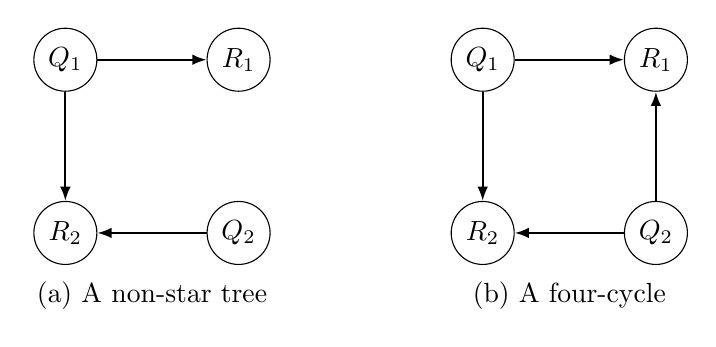
\begin{tikzpicture}[
  vertex/.style={circle,draw,minimum size=8mm,inner sep=1pt},
  edge/.style={-{Latex[length=1.8mm]},thick}]
\begin{scope}
\node[vertex] (q1) at (0,1.1) {$Q_1$};
\node[vertex] (r1) at (2.2,1.1) {$R_1$};
\node[vertex] (r2) at (0,-1.1) {$R_2$};
\node[vertex] (q2) at (2.2,-1.1) {$Q_2$};
\draw[edge] (q1.east)--(r1.west);
\draw[edge] (q1.south)--(r2.north);
\draw[edge] (q2.west)--(r2.east);
\node at (1.1,-1.9) {(a) A non-star tree};
\end{scope}
\begin{scope}[xshift=5.3cm]
\node[vertex] (cq1) at (0,1.1) {$Q_1$};
\node[vertex] (cr1) at (2.2,1.1) {$R_1$};
\node[vertex] (cr2) at (0,-1.1) {$R_2$};
\node[vertex] (cq2) at (2.2,-1.1) {$Q_2$};
\draw[edge] (cq1.east)--(cr1.west);
\draw[edge] (cq1.south)--(cr2.north);
\draw[edge] (cq2.west)--(cr2.east);
\draw[edge] (cq2.north)--(cr1.south);
\node at (1.1,-1.9) {(b) A four-cycle};
\end{scope}
\end{tikzpicture}
\end{adjustbox}
\caption{Two-step supports. Every arrow starts at a quotient factor
\(Q_j\) and ends at a subbundle factor \(R_i\).
The undirected path in (a) is not a star; the cycle in (b) has
no composable arrows.}
\label{fig06:supports}
\end{figure}


\subsection{Trees have cut-determined weights}

Suppose the undirected support is a tree. Deleting an edge \(e\)
leaves two components; let \(C_e\) be the one containing its target.
Summing \(Dk=b\) over this component gives
\begin{equation}\label{eq06:tree}
 k_e=b_{C_e}.
\end{equation}
Thus the balanced conductances are determined by the demands.
The harmonic coefficients affect the balancing potential and the
model metric, but not the leading spectrum.

Conversely, the \(m-1\) edge columns of the incidence matrix of
a tree form a basis of the zero-sum vertex space. A demand lies
in the strict stable cone exactly when all the cut values
in~\eqref{eq06:tree} are positive. Theorem~\ref{thm01:main}
therefore supplies a completely slope-determined operator on that
cone, with no restriction on the ratios of those cut values.
This includes the non-star path in Figure~\ref{fig06:supports}(a).
It does not include a higher-step filtration with composable arrows.

\subsection{Cycles retain harmonic orbit data}

For a connected graph, the cycle space is \(\ker D\), of
dimension \(|\Gamma(1)|-m+1\). Pairing
\(\log k-\log c=D^Tx_0\) with an integral cycle vector \(a\)
gives
\begin{equation}\label{eq06:cycle}
 \prod_e k_e^{a_e}=\prod_e c_e^{a_e}.
\end{equation}
For a bipartite cycle the nonzero coefficients of \(a\) alternate
between \(1\) and \(-1\). A basis of such identities, together
with \(Dk=b\), characterizes the balanced positive vector:
if the cycle identities hold, then
\(\log k-\log c\) lies in \((\ker D)^\perp=\operatorname{im}D^T\),
and uniqueness of balancing applies.

The right side of~\eqref{eq06:cycle} is invariant under scalar
changes of the factor metrics, because those multiply \(c\)
by a vertex scaling. It records harmonic information about the
extension orbit. It is not determined by the incidence cone.

For the four-cycle with unit masses and
\(b=\rho(1,1,-1,-1)\), the row and column sums force
\[
 k=\rho
 \begin{pmatrix}a&1-a\\1-a&a\end{pmatrix}.
\]
Writing \(\theta=c_{11}c_{22}/(c_{12}c_{21})\), the cycle
identity gives
\[
 \frac{a^2}{(1-a)^2}=\theta,\qquad
 a=\frac{\sqrt\theta}{1+\sqrt\theta}.
\]
In vertex order \((R_1,R_2,Q_1,Q_2)\), the constant vector is
the null vector. The other three vectors
\[
 (1,-1,-1,1),\qquad (1,-1,1,-1),\qquad(1,1,-1,-1)
\]
have eigenvalues, respectively,
\begin{equation}\label{eq06:fourcycle}
 2\rho a,\qquad 2\rho(1-a),\qquad2\rho.
\end{equation}
Changing \(\theta\) changes the leading coefficients with the
same masses and demands. Harmonic coefficients cannot therefore
be discarded from the general cyclic theorem.

The geometric family below has an additional reference symmetry
which fixes its cycle ratio. That simplification is a property of
the chosen geometric and metric data, not of the chamber alone.

\subsection{Freezing the coefficients}

Let \(k^{(0)}(b(s))\) denote balancing at the actual demand
\(b(s)\) with the reference coefficients \(c(0)\).
Smoothness and Proposition~\ref{prop02:coefficient} give
separate edge comparisons with relative error \(O(|s|)\).
Min--max and Theorem~\ref{thm01:main} yield
\begin{equation}\label{eq06:frozen}
 \lambda_j(h_{\mathrm{HE},s})
 =\nu_j(k^{(0)}(b(s)))
       \bigl(1+O(\sigma(s)+|s|)\bigr),\qquad 1\leq j<m.
\end{equation}
The constants remain independent of positive demand ratios.
An \(O(\sigma)\) formula with frozen coefficients requires an
additional geometric reason for \(|s|=O(\sigma)\). We will
verify such a reason in the tangent example.

\subsection{A spanning-tree expression}

For a connected graph let
\[
 \mathcal T_\Gamma(k)=
 \sum_{\substack{T\subset\Gamma\\T\text{ a spanning tree}}}
                  \prod_{e\in T}k_e
\]
be its weighted spanning-tree polynomial.
The following finite identity is classical; we give the proof to
make the rank normalization explicit. For a primary account of
the more general all-minors identity, see~\cite{zernik2013}.

\begin{proposition}\label{prop06:product}
The positive eigenvalues of~\eqref{eq01:graphoperator} satisfy
\begin{equation}\label{eq06:finiteproduct}
 \prod_{j=1}^{m-1}\nu_j(k)
 =\frac{\sum_vr_v}{\prod_vr_v}\mathcal T_\Gamma(k).
\end{equation}
Consequently the actual Hermitian--Einstein small cluster obeys
\begin{equation}\label{eq06:actualproduct}
 \prod_{j=1}^{m-1}\lambda_j(h_{\mathrm{HE},s})
 =\frac{R}{\prod_vr_v}\mathcal T_\Gamma(k(s,b(s)))
                         \bigl(1+O(\sigma(s))\bigr).
\end{equation}
\end{proposition}

\begin{proof}
Delete one row \(i\) of the incidence matrix. Cauchy--Binet
expresses the corresponding principal cofactor of \(L_k\) as
\[
 \sum_{\substack{T\subset\Gamma(1)\\|T|=m-1}}
       \det(D_{\widehat i,T})^2\prod_{e\in T}k_e.
\]
The reduced incidence determinant is zero unless \(T\) is a
spanning tree, and is \(1\) or \(-1\) for a tree. The zero
case follows from a cycle dependence or disconnectedness;
the tree case follows by successively removing leaves.
Thus every such cofactor is \(\mathcal T_\Gamma(k)\).

The matrix \(A(k)=M^{-1/2}L_kM^{-1/2}\) has null vector
\(z=(\sqrt{r_v})_v\), with \(\|z\|^2=R\).
Its adjugate is
\[
 \operatorname{adj} A
 =\frac{\prod_{j<m}\nu_j}{R}\,zz^*.
\]
The \(i\)-th diagonal cofactor is therefore
\((r_i/R)\prod_{j<m}\nu_j\). On the other hand it equals
\(\mathcal T_\Gamma(k)/\prod_{v\ne i}r_v\).
Equating these expressions proves~\eqref{eq06:finiteproduct}.
The individual relative estimates give~\eqref{eq06:actualproduct},
since the number of factors is fixed.
\end{proof}

For a tree the polynomial is a single monomial, and
\eqref{eq06:tree} expresses every factor as a cut margin.
For the four-cycle at \(\theta=1\), each edge has weight
\(\rho/2\); its four spanning trees give
\(\mathcal T_\Gamma=\rho^3/2\).
The unit-mass positive eigenvalue product is \(2\rho^3\),
as in~\eqref{eq06:fourcycle}. With masses \((1,2,3,5)\)
and \(\rho=1\), the product instead equals \(11/60\).
The rank factor in~\eqref{eq06:finiteproduct} is essential.

The product in~\eqref{eq06:actualproduct} concerns only the
small cluster. It neither computes a zeta-regularized determinant
of the full elliptic operator nor supplies its high-frequency
asymptotics.

% ============================================================
% section_07_geometry.tex
% ============================================================
\section{A tangent bundle with three independently separated scales}
\label{sec07:geometry}

We finish with a genuine tangent bundle. The example has a four-cycle
support, full local slope coordinates, and a square-cone stable
chamber. A reference symmetry removes its cycle coefficient from
the leading spectrum. This lets us realize three distinct spectral
orders on one fixed bundle and a smooth family of ample forms.

\subsection{The fourfold and its tangent sequence}

Let
\[
 B=\PP^1\times\PP^1,\qquad L=\mathcal O_B(1,-1),\qquad
 X=\PP_B(\mathcal O_B\oplus L)
            \times_B\PP_B(\mathcal O_B\oplus L),
\]
where projectivization parametrizes one-dimensional quotients.
Write \(\pi:X\to B\), let \(h_1,h_2\) be the pulled-back
hyperplane classes, and let \(\xi_1,\xi_2\) be the tautological
classes. Set
\[
 \ell=h_1-h_2,\qquad \eta_i=\xi_i-\ell/2.
\]
This is a smooth projective toric fourfold of Picard rank four.
For an explicit description, in a lattice basis \(e_1,e_2,f_1,f_2\)
its ray pairs are
\[
 \{e_1,-e_1\},\quad\{e_2,-e_2\},\quad
 \{f_1,-f_1+e_1+e_2\},\quad
 \{f_2,-f_2-e_1-e_2\}.
\]
Here \(e_i\) is the fibre direction of the \(i\)-th projective
bundle and \(f_j\) the \(j\)-th base direction. The divisors of
the pair \(\{e_i,-e_i\}\) have classes \(\xi_i\) and
\(\xi_i-\ell\); both divisors in the \(j\)-th base pair have
class \(h_j\). A maximal cone chooses one ray from each pair; every resulting
basis is unimodular.

For a real divisor \(H=x\eta_1+y\eta_2+uh_1+vh_2\), the
ample inequalities are
\begin{equation}\label{eq07:ample}
 x,y>0,\qquad u,v>(x+y)/2.
\end{equation}
Here is a direct verification. The divisor polytope has inequalities
\[
 \begin{gathered}
 -x/2\leq t_1\leq x/2,\qquad
 -y/2\leq t_2\leq y/2,\\
 -u/2\leq q_1\leq u/2+t_1+t_2,\qquad
 -v/2\leq q_2\leq v/2-t_1-t_2.
 \end{gathered}
\]
Under~\eqref{eq07:ample}, all intervals have positive length
and the normal fan is precisely the displayed fan.
Conversely, the invariant fiber curves have degrees \(x,y\),
and the minimum degrees of base curves over the four fiber
sections are \(u-(x+y)/2\), \(v-(x+y)/2\).
Positivity on these curves forces~\eqref{eq07:ample}.

The tangent sequence of the smooth fiber product is
\begin{equation}\label{eq07:tangent}
 0\longrightarrow R_1\oplus R_2\longrightarrow T_X
          \longrightarrow Q_1\oplus Q_2\longrightarrow0,
\end{equation}
where
\[
 R_i=\mathcal O_X(2\xi_i)\otimes\pi^*L^{-1},\qquad
 Q_j=\pi^*\mathcal O_B(2h_j).
\]
Their first Chern classes \(2\eta_1,2\eta_2,2h_1,2h_2\)
form a basis of \(N^1(X)_\RR\), so the line bundles are distinct.

Every component of~\eqref{eq07:tangent} is nonzero.
Indeed, trivialize \(L\) with transition functions \(g_{ab}\).
An affine projective coordinate transforms as
\(z_{i,b}=g_{ab}^{\pm1}z_{i,a}\). Differentiation gives the
off-diagonal tangent cocycle
\[
 \pm d\log(g_{ab})\otimes z_i\partial_{z_i}.
\]
The Cartan field \(z_i\partial_{z_i}\) spans the
\(\mathcal O_B\)-summand in
\(\pi_*R_i=L^{-1}\oplus\mathcal O_B\oplus L\);
higher direct images vanish because \(R_i\) has nonnegative
degree on each fiber factor. The \(j\)-th base component
therefore has, in the corresponding direct summand
\[
 H^1(B,\mathcal O_B(-2h_j))
 \subset H^1(X,R_i\otimes Q_j^{-1}),
\]
the nonzero coefficient \(1\) or \(-1\) of \(c_1(L)\).
This proves complete four-cycle support for the actual tangent
extension, rather than for an abstract graph realization.

\subsection{An actual ample equal-slope class}

The intersection ring has relations
\[
 h_1^2=h_2^2=0,\qquad
 \eta_i^2=\ell^2/4=-h_1h_2/2,\qquad
 \int_X\eta_1\eta_2h_1h_2=1.
\]
Thus, for \(H_r=\eta_1+\eta_2+r(h_1+h_2)\),
\begin{equation}\label{eq07:degrees}
 H_r^4=24r^2-4,\qquad
 c_1(R_i)H_r^3=12r^2-4,\qquad
 c_1(Q_j)H_r^3=12r.
\end{equation}
Equality of the four line slopes occurs at
\begin{equation}\label{eq07:wall}
 r_*=\frac{3+\sqrt{21}}6>1,\qquad
 H_0=\eta_1+\eta_2+r_*(h_1+h_2).
\end{equation}
This is a real ample class, not an integral polarization.
At the wall,
\[
 H_0^4=16+4\sqrt{21},\qquad
 c_1(R_i)H_0^3=c_1(Q_j)H_0^3=6+2\sqrt{21}.
\]
All four line factors are stable and equal-slope there.
They meet every hypothesis of Theorem~\ref{thm01:main}.

The anticanonical class is
\(-K_X=2(\eta_1+\eta_2+h_1+h_2)\).
It is nef and big, but is on the boundary in~\eqref{eq07:ample},
so \(X\) is weak Fano and not Fano. No Fano or
Kähler--Einstein assertion is used in the example.

We need a full chart of demands, not just the one-parameter
classes \(H_r\).
Let \(C_v\) be the four factor Chern classes and
\(K_v=C_v-\frac14\sum_w C_w\).
The \(K_v\) span the three-dimensional primitive hyperplane
at \(H_0\), because the \(C_v\) are independent and
\(K_vH_0^3=0\).
The real ample Hodge index theorem makes the pairing
\(A,B\mapsto ABH_0^2\) negative definite on that hyperplane;
see~\cite[Theorem 6.4 and Corollary 6.5]{grebrosstoma2016}.
It follows that the centered slope derivative has rank three
and kernel \(\RR H_0\).

Volume changes nontrivially along that kernel:
\(dV(H_0)[H_0]=4V_0>0\).
The analytic inverse-function theorem on the hypersurface
\(V(H)=V_0\) therefore gives a full local chart
\begin{equation}\label{eq07:chart}
 H=H(s),\qquad b(H(s))=s,\qquad
 \sum_vs_v=0,\qquad V(H(s))=V_0.
\end{equation}
Choose a smooth Kähler representative family with
\(\|\omega_s-\omega_0\|_{C^a}=O_a(|s|)\), by taking bounded
closed representatives of divisor coordinates and shrinking
the chart. Such control is a choice of representatives, not
a consequence of fixed volume alone.

In vertex order \((R_1,R_2,Q_1,Q_2)\), put
\[
 x_i=b_{R_i},\qquad y_j=-b_{Q_j}.
\]
The positive incidence cone is exactly
\begin{equation}\label{eq07:chamber}
 x_1,x_2,y_1,y_2>0,\qquad
 x_1+x_2=y_1+y_2=\sigma.
\end{equation}
Necessity follows by summing incoming and outgoing weights;
the positive lift \(k_{ij}=x_i y_j/\sigma\) proves sufficiency.
Theorem~\ref{thm01:main} identifies this with the actual local
stable chamber of \(T_X\). Its closure is the semistable locus:
closed limits of stable polarizations satisfy each subsheaf
slope inequality, while a negative coordinate destabilizes via
a target line or the kernel of a source quotient.
The section \(\sigma=1\) of the closed demand cone is a square,
so it is nonsimplicial. The full polarization space has the
additional free volume coordinate.

\subsection{A symmetry which determines the leading weights}

The involution exchanging the two projective factors preserves
\(H_0\). Choose an invariant Kähler representative \(\omega_0\)
by averaging. Choose compatible factor Hermitian--Einstein
metrics: exchange the two \(R_i\) metrics, and take invariant
metrics on \(Q_j\).
The tangent sequence is natural under this involution, which
exchanges its two Cartan extension classes for each fixed \(j\).
Pullback is unitary on the coefficient Dolbeault complexes.
It commutes with the differential and its adjoint, so uniqueness
of harmonic representatives gives
\[
 c_{1j}(0)=c_{2j}(0)=q_j>0.
\]
Scalar changes of the factor metrics allow the equivalent form
\(c_{ij}(0)=a_iq_j\), without changing any cycle ratio.
The reference cycle ratio is therefore one.

Only the reference form was required to be invariant. The full
chart contains \(x_1\ne x_2\); its current coefficient array
need not have rank one.
Smoothness gives
\(\log(c_{ij}(s)/c_{ij}(0))=O(|s|)\).
On the stable part of~\eqref{eq07:chart},
\(\|s\|_1=2\sigma\), so this error is \(O(\sigma)\).
Balancing the reference coefficients yields
\begin{equation}\label{eq07:explicitgraph}
 k^0_{ij}=\frac{x_i y_j}{\sigma},\qquad
 L^0=
 \begin{pmatrix}
 \diag(x)&-xy^T/\sigma\\
 -yx^T/\sigma&\diag(y)
 \end{pmatrix}.
\end{equation}
Proposition~\ref{prop02:coefficient} and
Theorem~\ref{thm01:main} imply
\[
 \lambda_j(h_{\mathrm{HE},s})
 =\nu_j(L^0(s))(1+O(\sigma)),\qquad 1\leq j\leq3,
 \qquad \lambda_4\geq\gamma>0,
\]
uniformly through all positive facet ratios.
The symmetry fixes the cycle data, not the absolute \(q_j\).
For example, the diagonal metric still uses
\[
 w_{R_i}=x_i/a_i,\qquad w_{Q_j}=\sigma q_j/y_j,\qquad
 W_v=w_v/\Bigl(\prod_ww_w\Bigr)^{1/4}.
\]
The model \(\Phi_s^*(\bigoplus_vW_vh_{v,s})\) has the same
determinant as the actual metric and satisfies
\eqref{eq01:metric}. Thus the spectral simplification does not
discard the harmonic information needed to describe metrics.

\subsection{Three spectral orders on the fixed tangent bundle}

For \(0<\varepsilon\ll1\), prescribe the demands
\begin{equation}\label{eq07:threeorders}
 x_1=\varepsilon^3,\quad x_2=\varepsilon,\quad
 y_1=\varepsilon^2,\quad
 y_2=\varepsilon-\varepsilon^2+\varepsilon^3.
\end{equation}
They lie in~\eqref{eq07:chamber} and are realized by the actual
ample chart~\eqref{eq07:chart}.
Let \(\nu_1\leq\nu_2\leq\nu_3\) be the positive eigenvalues of
\eqref{eq07:explicitgraph}. Their elementary symmetric
functions satisfy
\begin{equation}\label{eq07:symmetric}
 e_1=2\varepsilon+O(\varepsilon^3),\qquad
 e_2=3\varepsilon^3(1+O(\varepsilon)),\qquad
 e_3=4\varepsilon^6(1+O(\varepsilon)).
\end{equation}
For direct verification on the balance hyperplane
\(x_1+x_2=y_1+y_2=\sigma\), if
\(S_x=x_1^2+x_2^2\), \(S_y=y_1^2+y_2^2\), then
\[
 e_1=2\sigma,\qquad
 e_2=\frac{4\sigma^2-S_x-S_y-2S_xS_y/\sigma^2}{2},
 \qquad
 e_3=\frac{4x_1x_2y_1y_2}{\sigma}.
\]
The last formula follows either by a principal cofactor or
from Proposition~\ref{prop06:product}.

These formulas separate the roots without selecting
eigensections. Since \(\nu_3\geq e_1/3\) and
\(e_2\geq\nu_3(\nu_1+\nu_2)\), we have
\(\nu_1+\nu_2=O(\varepsilon^2)\), hence
\(\nu_3=2\varepsilon(1+O(\varepsilon))\).
Next
\[
 \nu_1\nu_2=2\varepsilon^5(1+O(\varepsilon)),\qquad
 \nu_1+\nu_2=\tfrac32\varepsilon^2(1+O(\varepsilon)).
\]
Their product divided by the square of their sum is
\(O(\varepsilon)\), so the smaller root is negligible in the
sum. Therefore
\[
 \nu_1=\tfrac43\varepsilon^3(1+O(\varepsilon)),\quad
 \nu_2=\tfrac32\varepsilon^2(1+O(\varepsilon)),\quad
 \nu_3=2\varepsilon(1+O(\varepsilon)).
\]
The actual relative error is also \(O(\sigma)=O(\varepsilon)\).
Taking \(\varepsilon=t^2\) gives a smooth approach of actual
ample forms on which
\begin{equation}\label{eq07:actualthreeorders}
 \lambda_1=\tfrac43t^6(1+O(t^2)),\qquad
 \lambda_2=\tfrac32t^4(1+O(t^2)),\qquad
 \lambda_3=2t^2(1+O(t^2)),\qquad
 \lambda_4\geq\gamma.
\end{equation}
The trace-free \(L^2\) inverse norm consequently grows as
\(\frac34t^{-6}(1+O(t^2))\).
These are endomorphism energies and a linear inverse norm;
nonlinear metric-response and actual-flow conclusions
require separate arguments.

The same line factors also give a non-star tree example on
this fourfold. Retain three of the four nonzero tangent
extension components and set the fourth to zero.
The resulting holomorphic extension remains integrable and has
the path support in Figure~\ref{fig06:supports}(a).
It need not be the tangent bundle, but the full demand chart
and Theorem~\ref{thm01:main} apply to it. Its leading weights
are the three cut sums in~\eqref{eq06:tree}. For the path
\(Q_1\to R_1\), \(Q_1\to R_2\), \(Q_2\to R_2\), these
are \(x_1\), \(y_1-x_1\), and \(y_2\). Its stable chamber is
therefore the subcone \(y_1>x_1\) of \eqref{eq07:chamber}.

The higher-dimensional products
\(\PP_B(\mathcal O\oplus\mathcal O(1^k,-1^k))
\times_B\PP_B(\mathcal O\oplus\mathcal O(1^k,-1^k))\),
with \(B=(\PP^1)^{2k}\), lead to the broader geometric
realization problem. The fourfold already shows how the
same actual bundle can carry chamber, extension, and complete
small-spectrum descriptions. Its construction uses no
metric-response or dynamical theorem as a premise.

% ============================================================
% section_08_scope.tex
% ============================================================
\section{Scope and supporting calculations}\label{sec08:scope}

The analytic mechanism proved here has three ingredients: a finite
parallel algebra at the graded bundle, a uniformly invertible
elliptic complement, and curvature identities which control the
remaining error at each weak cut. In the distinct-factor two-step
case, the parallel algebra is the scalar vertex space and every
amplitude assignment is integrable. This is the setting in which
the graph description has been justified throughout the whole
positive chamber.

Repeated stable factors replace the scalar parallel space by a
matrix algebra. Composable arrows require an integrability
equation, and singular graded sheaves require a different analytic
setting. The present theorem does not resolve those problems.
Nor does its finite cluster product compute the determinant of
the full elliptic operator.

The tree and cyclic examples distinguish the information needed
for a quantitative theory. On trees, ranks and slope demands
determine the leading spectrum. Cycles can retain harmonic orbit
data, while actual model metrics retain harmonic coefficients
even when a symmetry simplifies the spectrum. These distinctions
remain necessary when the spectral construction is combined
with geometric realizability or with metric and flow estimates.
The latter require their own parameter and dynamical arguments.

All finite data used above can be checked directly from the
printed matrices and intersection relations. The accompanying
exact-arithmetic programs also recompute the path counterexample,
the four-cycle eigenvectors, the nonunit-rank product, the
fourfold intersections and the three-scale symmetric
coefficients.\footnote{The sources are
\texttt{figures/code/compute06\_graphs.py} and
\texttt{figures/code/compute07\_tangent.py}; they require only
the Python standard library. The support diagram is given by
\texttt{figures/code/fig06\_supports.tex}.}
Their records use rational arithmetic and the exact field
\(\mathbb Q(\sqrt{21})\). They provide reproducible finite
calculations, not numerical solutions of the
Hermitian--Einstein equation. The metric existence, relative
spectral estimates and geometric parameter identifications
are established by the proofs above.

% ============================================================
% BIBLIOGRAPHY
% ============================================================
\begin{thebibliography}{Wue26a}
\bibitem[CT24]{clarketipler2024}
A.~Clarke and C.~Tipler,
\emph{Semi-stability and local wall-crossing for Hermitian Yang--Mills connections},
J.\ Symplectic Geom.\ \textbf{22} (2024), no.~3, 673--694; arXiv:2304.05245.

\bibitem[Del25]{delloque2025}
R.~Delloque,
\emph{Continuity of HYM connections with respect to metric variations},
J.\ Lond.\ Math.\ Soc.\ (2) \textbf{112} (2025), no.~1, e70219;
arXiv:2403.16814v4.

\bibitem[GRT16]{grebrosstoma2016}
D.~Greb, J.~Ross, and M.~Toma,
\emph{Variation of Gieseker moduli spaces via quiver GIT},
Geom.\ Topol.\ \textbf{20} (2016), no.~3, 1539--1610;
arXiv:1409.7564v2.

\bibitem[Kob87]{kobayashi1987}
S.~Kobayashi,
\emph{Differential Geometry of Complex Vector Bundles},
Publications of the Mathematical Society of Japan \textbf{15},
Kan\=o Memorial Lectures \textbf{5},
Iwanami Shoten and Princeton Univ.\ Press, 1987.

\bibitem[NZ13]{zernik2013}
A.~Netser Zernik,
\emph{Taylor expansion proof of the matrix tree theorem---Part II},
arXiv:1308.2160v1 (2013).

\bibitem[ST24]{sektnantipler2024}
L.~M.~Sektnan and C.~Tipler,
\emph{Hermitian Yang--Mills connections on pullback bundles},
Calc.\ Var.\ Partial Differential Equations \textbf{63} (2024), no.~1,
Paper No.~13, 63~pp.; arXiv:2006.06453v2.

\bibitem[Wue26a]{wuebben2026walls}
B.~J. Wuebben,
\emph{Small Dolbeault eigenvalues near stability walls},
preprint, 2026; \href{https://doi.org/10.5281/zenodo.23682045}{Zenodo:23682045}.
\end{thebibliography}

\bigskip
\noindent{\sc Bernd Johannes Wuebben, New York, NY,} \texttt{wuebben@gmail.com}

\end{document}
